\section{Overordnede sekvensdiagrammer}
Der er lavet enkelte system sekvensdiagrammer, for udvalgte user stories, der har særlig signifikans for systemmet. Figur \ref{fig:SDOpretBytteannoncedia} viser hvordan brugeren igennem systemet for oprettet en bytteannonce, på figur \ref{fig:SDOpretBrugerprofildia} ses hvordan brugeren kan oprette en brugerprofil og  på figur \ref{fig:SDSearchBarterAd} vises søgefunktionaliteten.

\begin{figure}[H]
	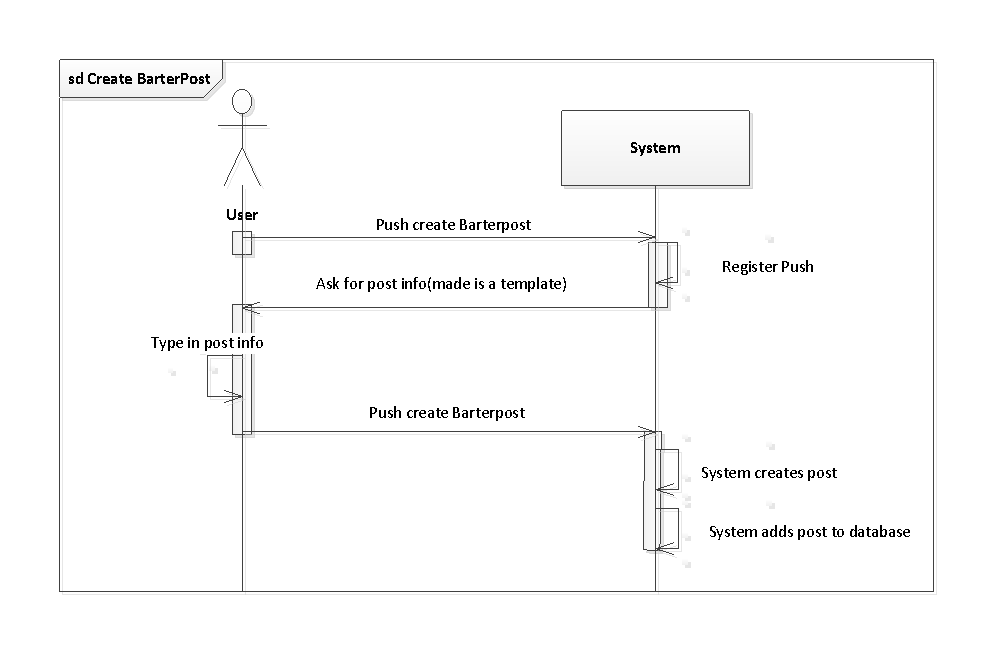
\includegraphics[trim = 6mm 6mm 6mm 6mm, clip, width=0.95\textwidth]{figures/SDOpretBytteAnnonce.PDF}
	\caption{Opretbytteannonce, System sekvensdiagram }
	\label{fig:SDOpretBytteannoncedia}
	\centering
\end{figure}

\noindent På figur \ref{fig:SDOpretBytteannoncedia} vises der hvordan en bruger skal oprette en annonce (BarterAd). Brugeren trykker på en knap "Opret bytteannonce"\ på hjemmesiden. Systemet registrer dette ved så at præsentere en formular, hvorved brugeren kan indtaste relevante oplysninger. Når brugeren så trykker "Opret", så registrerer systemet og opretter derefter en annonce, som bliver lagt på en database.
	
	
\begin{figure}[H]
	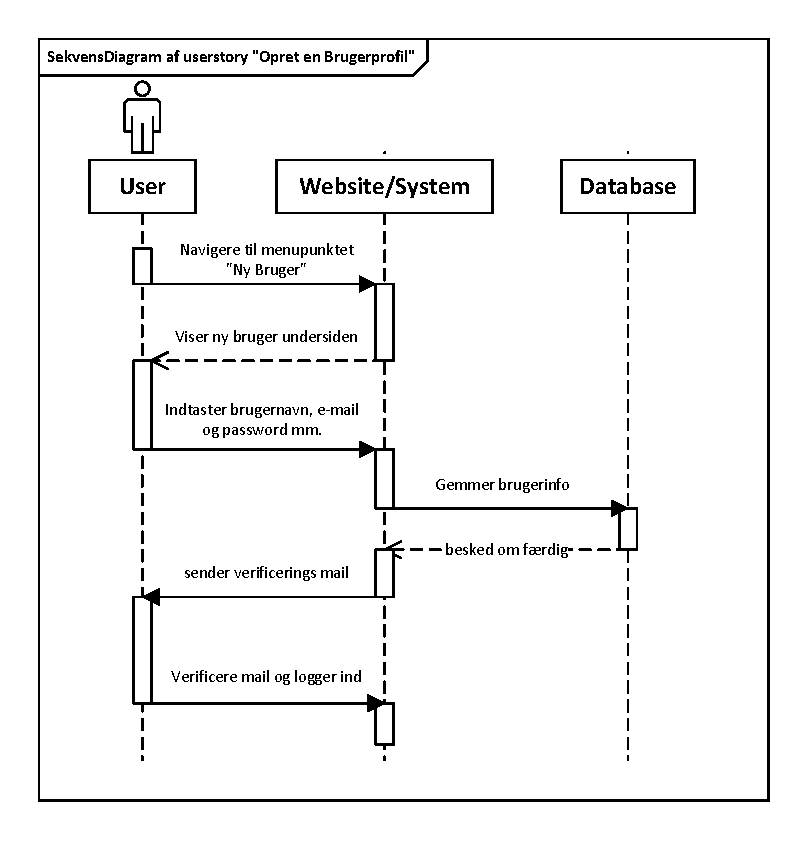
\includegraphics[trim = 6mm 6mm 6mm 6mm, clip, width=0.95\textwidth]{figures/SekvensdiagramOpretBrugerprofil.PDF}
	\caption{Opretbrugerprofildia, System sekvensdiagram }
	\label{fig:SDOpretBrugerprofildia}
\end{figure}

\noindent På figur \ref{fig:SDOpretBrugerprofildia} vises der hvordan en nu bruger skal registrere sig som ny bruger på hjemmesiden. Brugeren navigerer til menupunktet "Registrer bruger"\, systemet registrere dette og viser en formular for brugeren, hvor der kan indtastes relevante informationer. Informationen gemmes ned på en database og systemet sender en verifikations E-mail til brugeren. Brugeren verificere sin E-mail og kan nu logge ind.

\begin{figure}[H]
	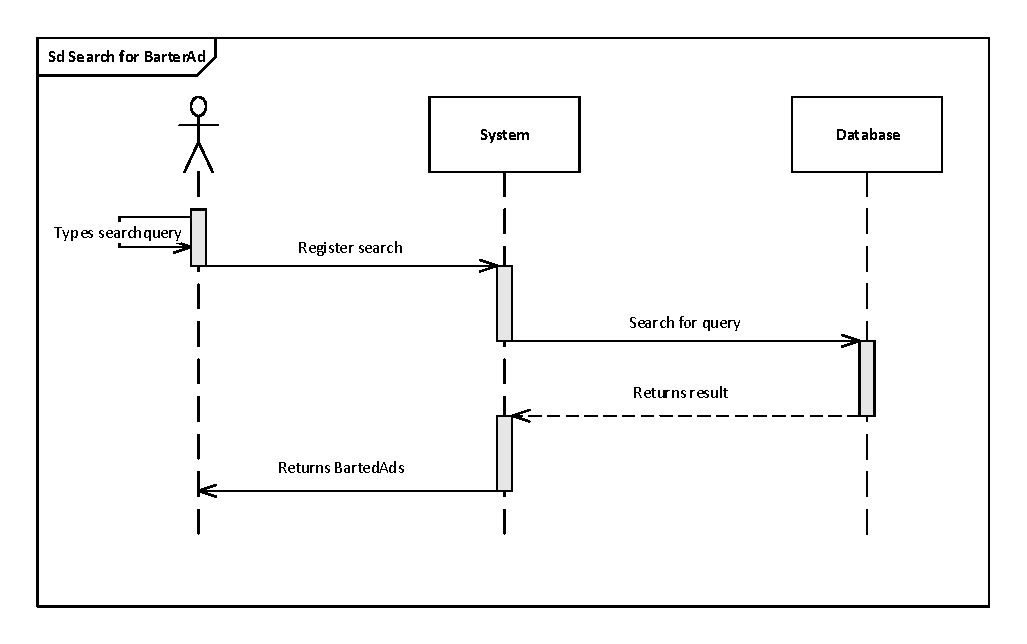
\includegraphics[trim = 6mm 6mm 6mm 6mm, clip, width=0.95\textwidth]{figures/SDSearchBartedAd.PDF}
	\caption{Opretbytteannonce, System sekvensdiagram }
	\label{fig:SDSearchBarterAd}
	\centering
\end{figure}

\noindent På figur \ref{fig:SDSearchBarterAd} vises der, hvordan en bruger søger efter noget bestemt. Brugeren indtaster et søgeord, som så sendes til systemet. Systemet søger så i databasen, hvor den så returner et resultat til systemet. Systemet præsenterer så  de BarterAds, der passer til brugerens søgeord. 